\documentclass[a4paper,12pt]{article}
\usepackage[pdftex]{graphicx}

\pagestyle{empty} \setlength{\parindent}{0mm}
\addtolength{\topmargin}{-0.5in} \setlength{\textheight}{9in}
\addtolength{\textwidth}{1in} \addtolength{\oddsidemargin}{-0.5in}

\begin{document}

{\bf Name:} Matt Forbes \\
{\bf Partner:} Stuart  \\ 
{\bf Section:} Phys 233 - Thursday \\
{\bf TA:} Ellis Roe  \\ \\ 
{\bf Lab 2:} Combining Waves \\

\section{Purpose}
For this lab, we experimented with the combination of waves of
different frequencies, and the properties of that resulting wave. The
lab was split in to three exercises. First of these was the
introduction to the FFT (Fast Fourier Transform) spectrum analyzer,
where we recorded the FFT of an input wave generated by a function
generator with sine, square, and sawtooth waves. Next, in exercise
two, our goal was to synthesize (construct) a compound wave by
combining individual waves of different frequencies and phase shifts
(cosine vs. sine.) Finally, in the third exercise, we were tasked with
simply observing different sound waves created by ourselves or various
devices made available to us. 

\section{Procedure}
Here, I will describe the procedure of each exercise separately. Note:
some details of each experiment may appear in the data section which
is needed to clarify what the data represents.

\subsection{Exercise 1}
For this exercise, we used: a function generator, voltage sensor, and
the Data Studio software configured both as an oscilloscope and FFT
analyzer. \\

Once the hardware and sensors were set up, our first task
was to set the function generator to create a sine wave with frequency
set at 220 Hz. To verify that are sensors were calibrated correctly,
we were to measure the period of the captured wave and verify that
this was indeed a 220 Hz wave. We also measured the relative
amplitudes and frequencies of the peaks. \\

Next, we worked with a square wave. Configuring the function generator
to create a square wave is as simple as pressing the square wave
button. Again, we took the same measurements on the FFT output:
relative amplitude and frequency of the peaks. \\ 

Finally, we repeated the measurements with a sawtooth wave, which like
the square wave, is a matter of pressing the sawtooth button on the
function generator.

\subsection{Exercise 2}
In exercise 1 we analyzed waves created by a function generator, and
here we created our own waves by adjusting the relative amplitudes of
the fundamental harmonics of a basic sine wave (at 440 Hz.) Our
equipment in this exercise was: an oscilloscope and fourier
synthesizer. \\

Our first task was to create a sawtooth wave. We used the first five
harmonics with the following relative amplitudes and phase shifts: \\

\begin{tabular}{r | c c c c c}
  Harmonic: & 1 & 2 & 3 & 4 & 5 \\
  \hline
  Amplitude: & 1.0 & 0.5 & 0.333 & 0.25 & 0.2 \\
  Phase Shift: & 0 & 180$^{\circ}$ & 0 & 180$^{\circ}$ & 0 \\
\end{tabular} \\ \\

First, we reset all the settings on the synthesizer to their default
values according to the instructions listed in the lab, and switched
off the SUMMING AMPLIFIER for each fundamental frequency. Now,
one-by-one, we went through the first five fundamental frequencies and
adjusted their relative amplitude according to the above table. Once
all the harmonics were added, we turned up the volume on the
synthesizer to hear the resulting sound wave and observed the summed
output on the oscilloscope. \\

For the second part of this exercise, we were giving the following
expression for the $n^{\text{th}}$ amplitudes of a square wave: 

\begin{center}
  \[A_n = \frac{1}{T} \int_0^T y(t) sin(\frac{n{\pi}t}{T})dt\]
\end{center}

Given that $y(t)$ is constant for a square wave, we were asked to find
the relative amplitudes of the first five terms. With these relative
amplitudes, we set the synthesizer accordingly and observed a square
wave in the oscilloscope.

\subsection{Exercise 3}
The instructions for this exercise were quite vague, but it involved
setting up a microphone to the input of an oscilloscope and observing
what types of waves different sounds produced. Second, we hooked up
another microphone to the Data Studio software to see the FFT output
of those same sounds. \\

From here we just explored different sounds that we could make, such
as monotone sounds, beeps from phones, etc.

\section{Data}
\subsection{Exercise 1}
As described in the procedure section, we measured the period of the
displayed wave from Data Studio, as well as the relative amplitudes
and frequencies of the peaks. The function generator was set at 220
Hz, and we measured a period of 0.005 $\pm$ 0.0005 units, when scaled
appropriatel, is equal to 250 Hz. So our measurement was entirely
accurate, but fairly close. \\

Here are the measurements of the peaks for the sine wave: \\

\begin{tabular}{c | c}
  Frequency & Relative Amplitude \\
  \hline
  221 $\pm$ 2 Hz & 1.0 \\
  442 $\pm$ 2 Hz & 0.375 $\pm$ 0.01 \\
  661 $\pm$ 2 Hz & 0.225 $\pm$ 0.01 \\
  881 $\pm$ 2 Hz & 0.16 $\pm$ 0.01 \\
  1101 $\pm$ 2 Hz & 0.12 $\pm$ 0.01 \\
  1183 $\pm$ 2 Hz & 0.08 $\pm$ 0.01 \\
\end{tabular} \\

Next we set the function generator to a square wave and recorded the
same types of measurements: \\

\begin{tabular}{c | c}
  Frequency & Relative Amplitude \\
  \hline
  229 $\pm$ 2 Hz & 1.0 $\pm$ 0.01 \\
  676 $\pm$ 2 Hz & 0.25 $\pm$ 0.01 \\
  1118 $\pm$ 2 Hz & 0.19 $\pm$ 0.01 \\
  1566 $\pm$ 2 Hz & 0.15 $\pm$ 0.01 \\
  2018 $\pm$ 2 Hz & 0.08 $\pm$ 0.01 \\
\end{tabular} \\

Finally, for the sawtooth wave: \\

\begin{tabular}{c | c}
  Frequency & Relative Amplitude \\
  \hline
  73 $\pm$ 2 Hz & 1.0 $\pm$ 0.01 \\
  132 $\pm$ 2 Hz & 0.63 $\pm$ 0.01 \\
  201 $\pm$ 2 Hz & 0.42 $\pm$ 0.01 \\
  258 $\pm$ 2 Hz & 0.23 $\pm$ 0.01 \\
  327 $\pm$ 2 Hz & 0.25 $\pm$ 0.01 \\
\end{tabular}

\subsection{Exercise 2}

\begin{center}
  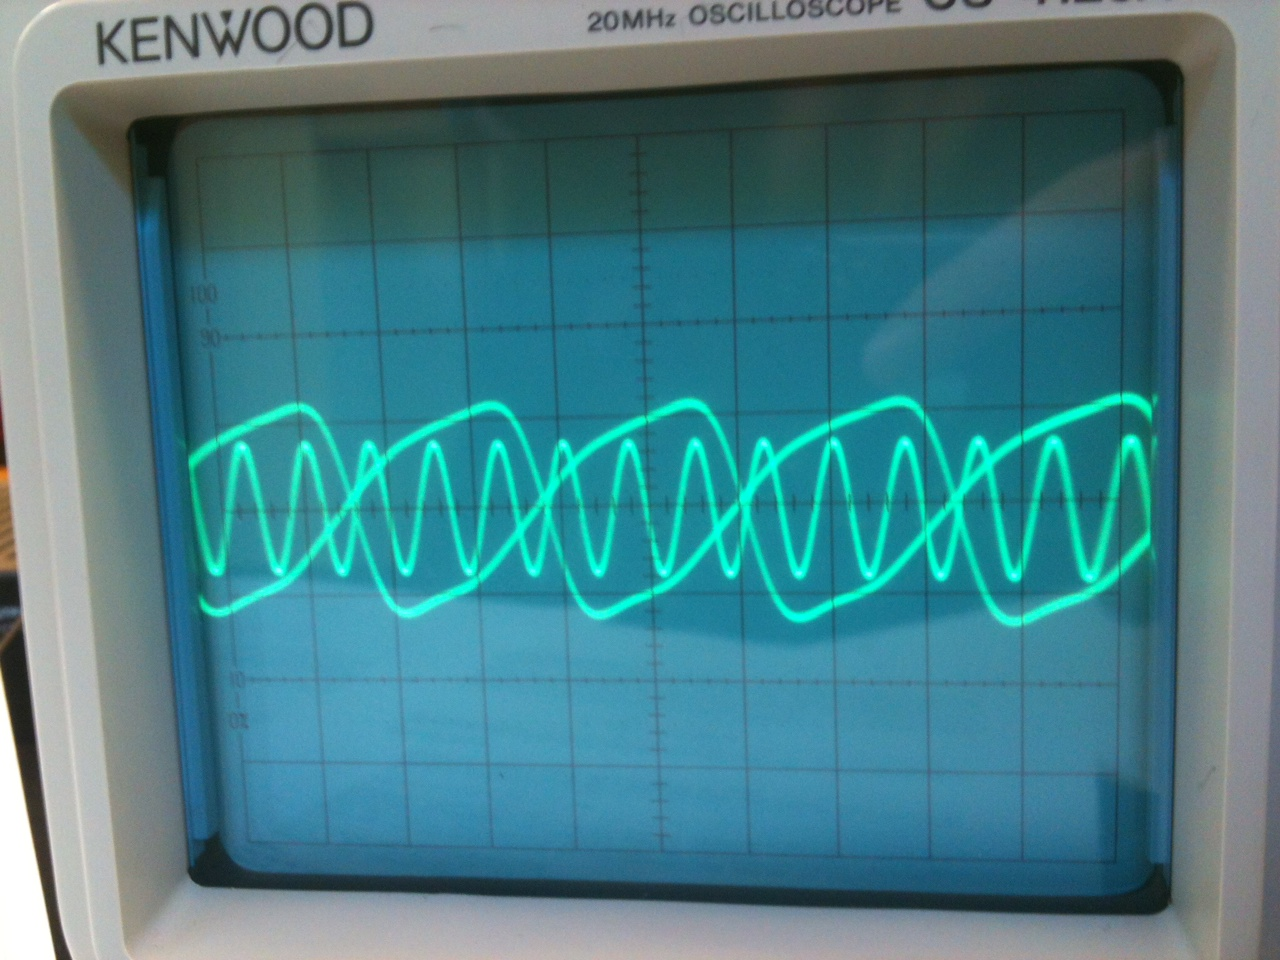
\includegraphics[width=3in]{photo1.jpg} \\
  
  The above photo is of the synthesized sawtooth wave. \\ \\
  
  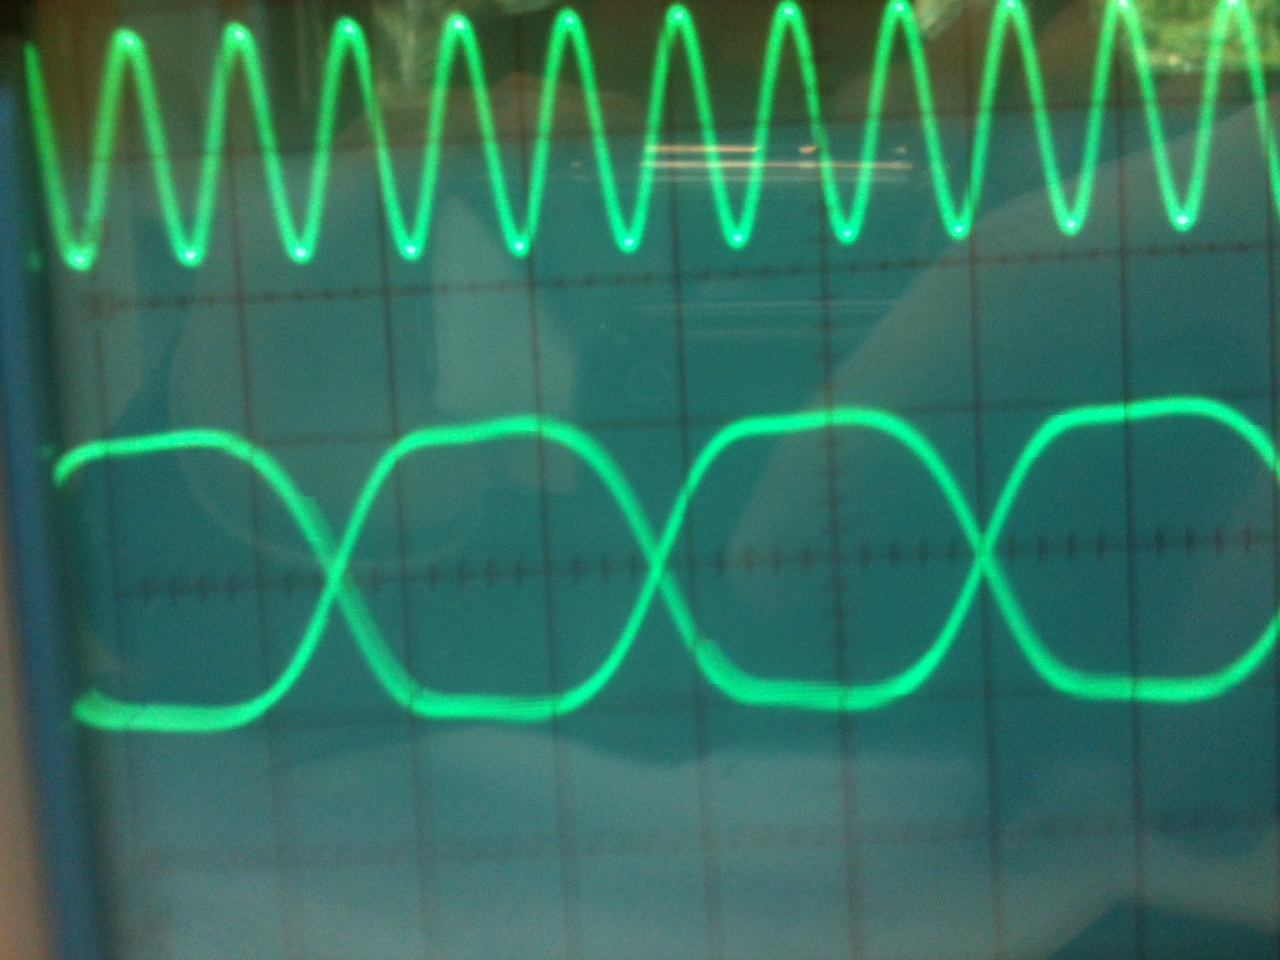
\includegraphics[width=3in]{photo2.jpg} \\
  
  The above photo is the synthesized square wave.
  \end{center} \\ \\

  
  Solving for $A_n$: \\
  
  \[
  A_n = \frac{1}{T}\int_0^T sin(\frac{n{\pi}t}{T})dt \\
  A_n = \frac{1}{n{\pi}}(-cos(n{\pi}) + 1) \\ \\
  
  A_1 = \frac{2}{{\pi}} = 1 \\
  A_2 = 0 \\
  A_3 = \frac{2}{3{\pi}} = \frac{1}{3} \\
  A_4 = 0 \\
  A_5 = \frac{2}{5{\pi}} = \frac{1}{5} \\
  \]
  
\subsection{Exercise 3}
\begin{tabular}{c | c}
  Frequency | Relative Amplitude \\
  \hline
  126 Hz & 0.8 \\
  253 Hz & 0.5 \\
  603 Hz & 0.5 \\
  628 Hz & 0.8 \\
  714 Hz & 0.5 \\
  761 Hz & 1.0 \\
  831 Hz & 0.6 \\
  882 Hz & 0.6 \\
\end{tabular}

(Note, frequencies are $\pm$ 2 Hz and amplitudes are $\pm$ 0.01) \\

\end{document}
